\section{Design Overview}\label{s:design}
\begin{figure}
    \centering
    \begin{subfigure}[b]{0.5\textwidth}
        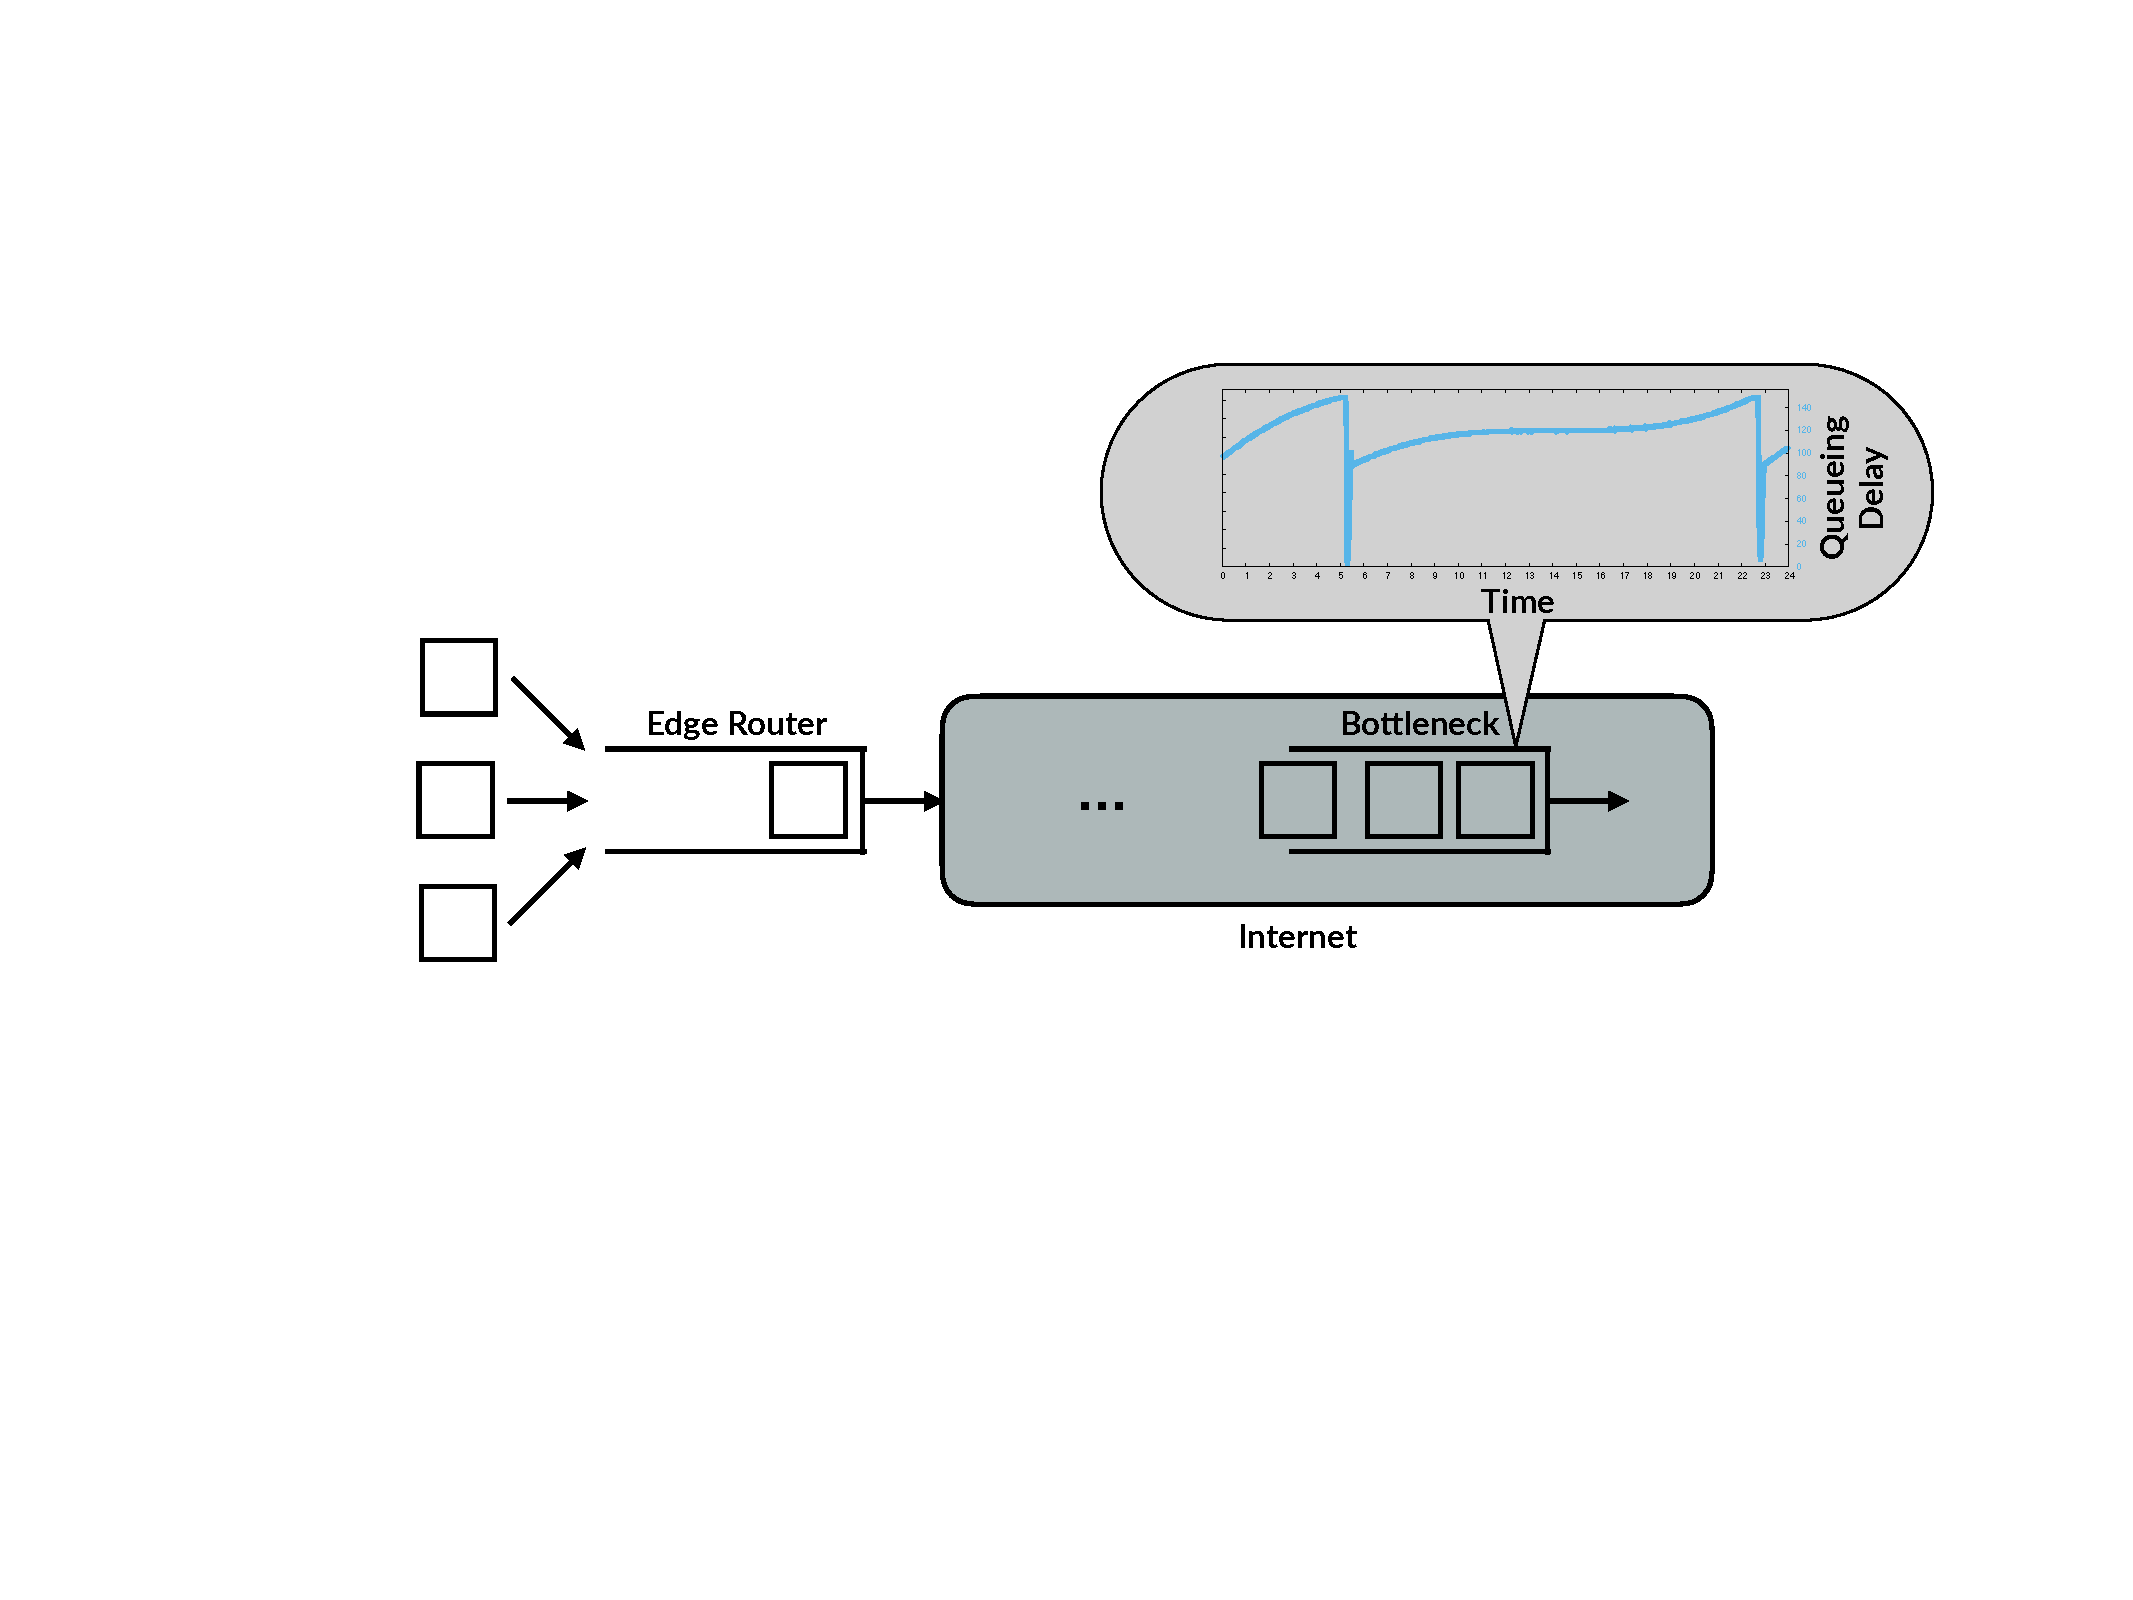
\includegraphics[width=\textwidth]{img/shift-bottleneck-before}
        \caption{Today, large queues can grow on congested routers that are outside the control of a domain.}\label{fig:design:shift-bottleneck:before}
    \end{subfigure}
    \begin{subfigure}[b]{0.5\textwidth}
        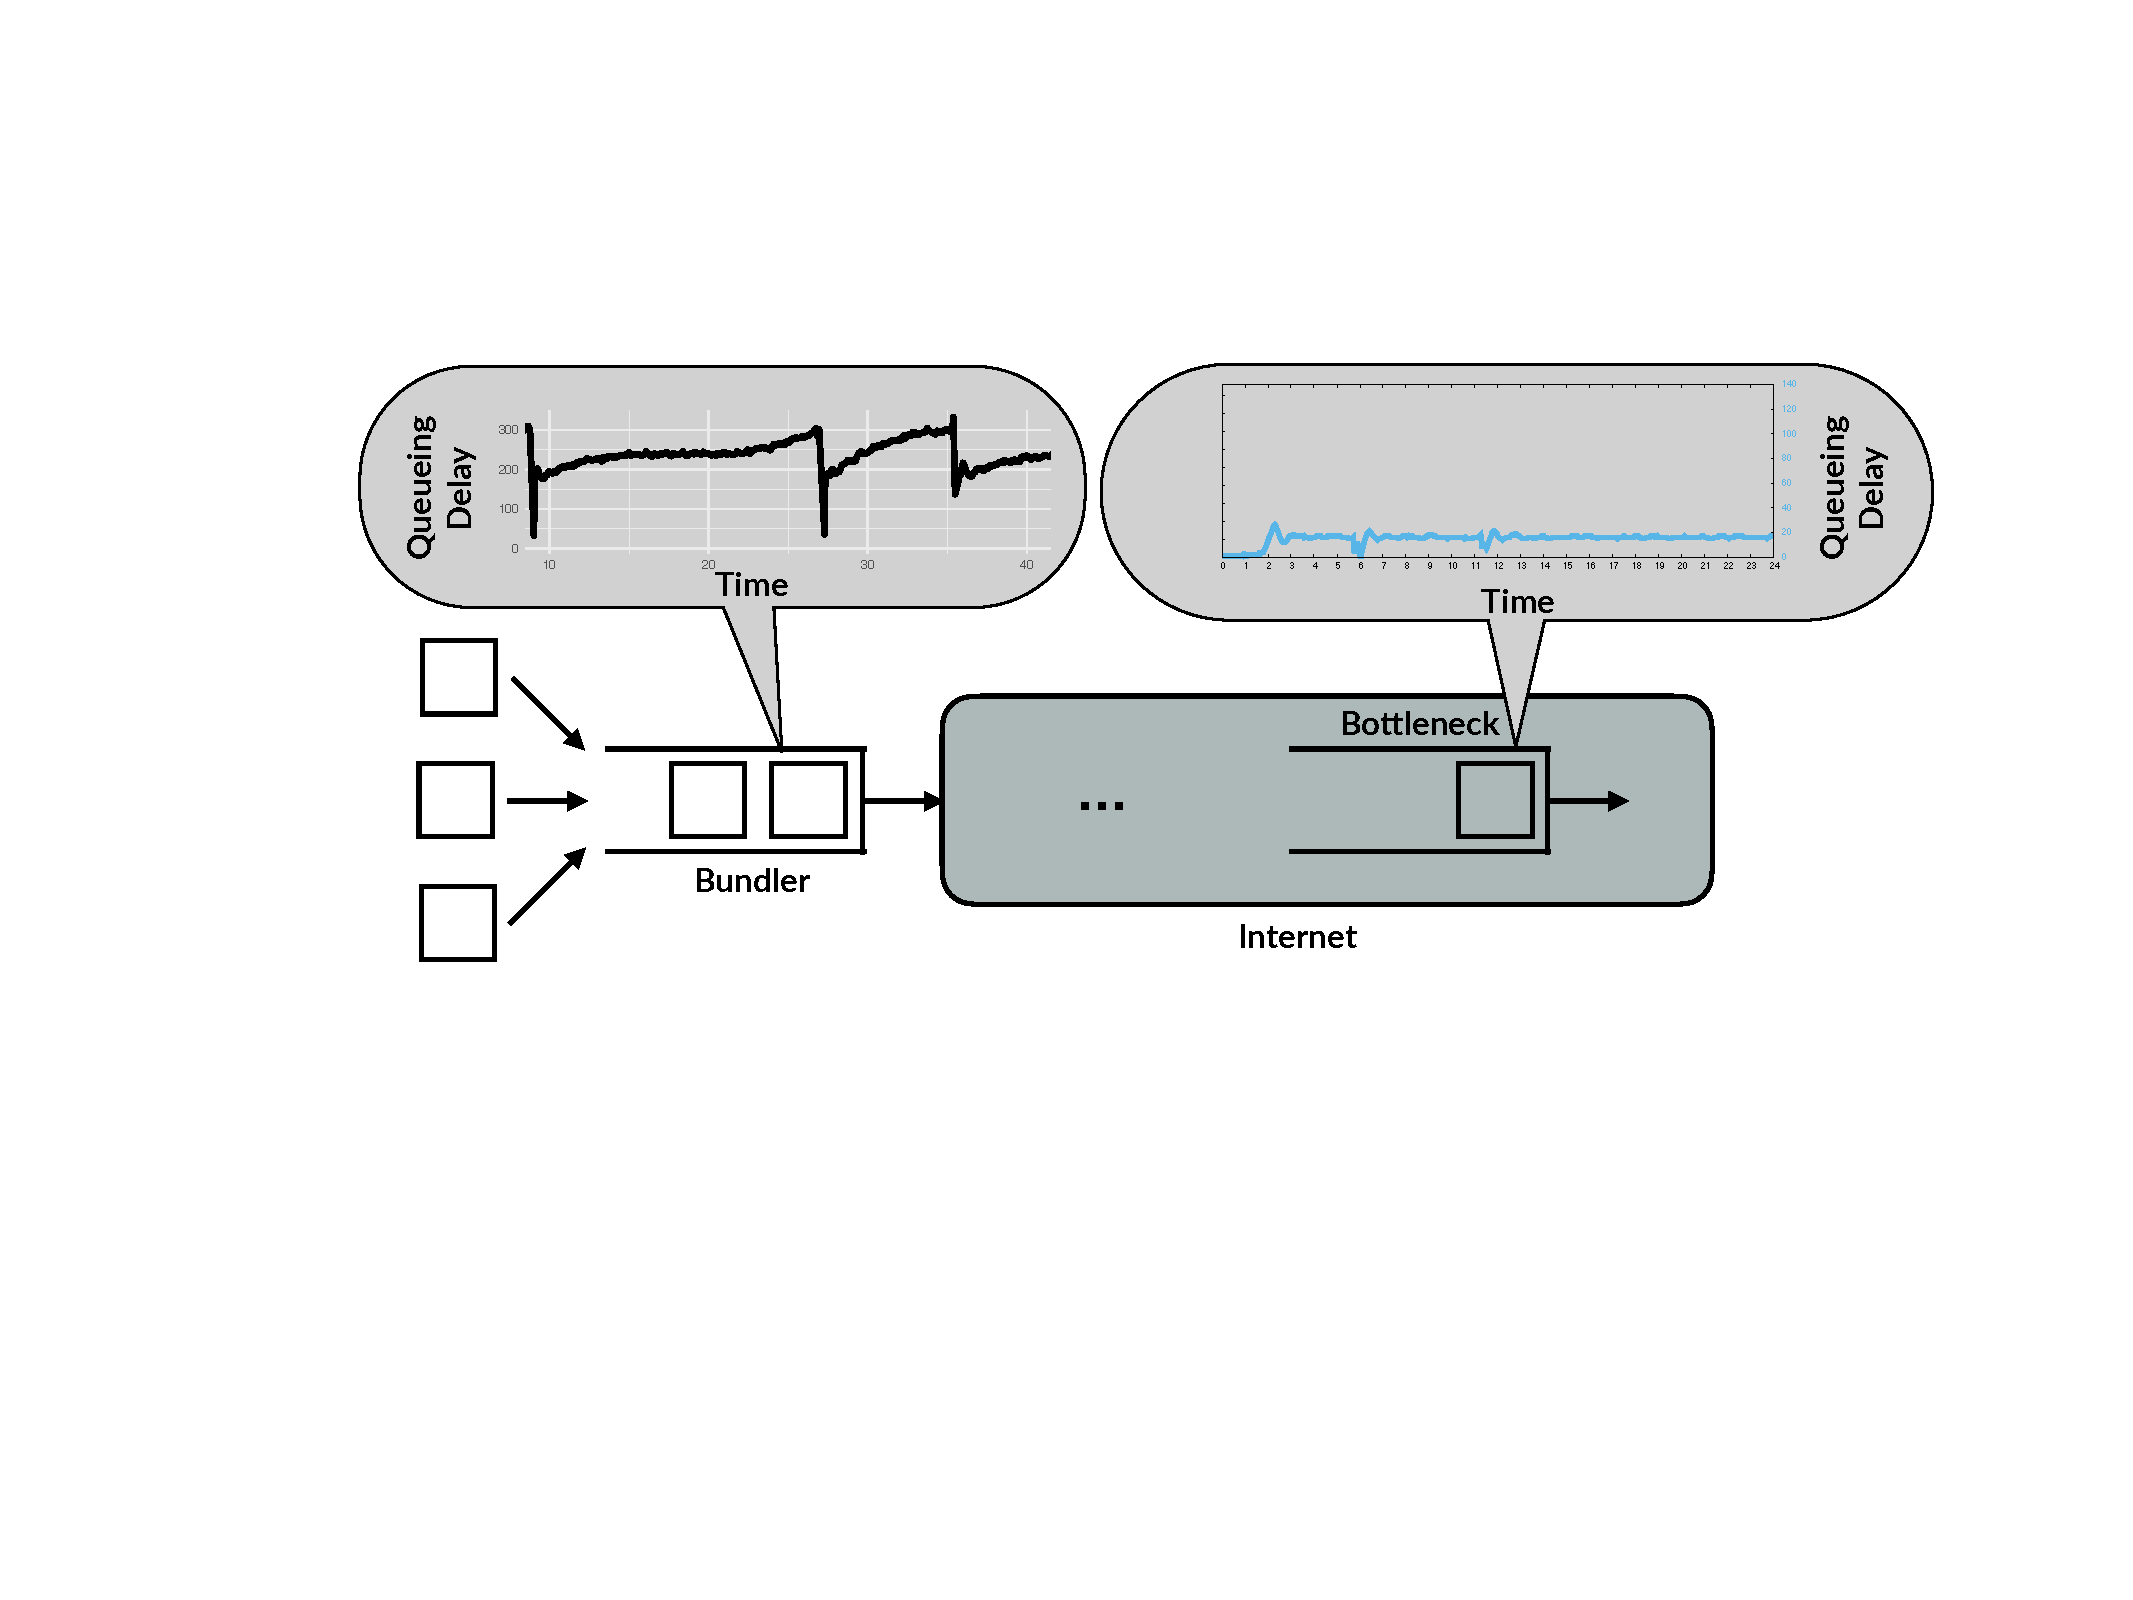
\includegraphics[width=\textwidth]{img/shift-bottleneck-after}
        \caption{\name can \emph{move} the bottleneck using a congestion control algorithm on the traffic aggregate.}\label{fig:design:shift-bottleneck:after}
    \end{subfigure}
    \caption{This illustrative example with a single flow and FIFO scheduling shows how \name can take control of queues in the network. The bubbles show the trend in measured queueing delays at the relevant queue over time. The queue where delays build up can best make scheduling decisions, since that is where there is the most choice between packets to send.}\label{fig:design:shift-bottleneck}
\end{figure}

\begin{outline}
\1 A \name has the following properties:
    \2 It measures congestion control information from the network path.
    \2 It enforces a pacing rate determined by a congestion control algorithm.
        \3 The congestion control algorithm takes as input measurements from the network path, and returns an aggregate rate at which \name should send its component traffic.
    \2 It provides a mechanism for scheduling the packets comprising the bundle.
\1 Simultaneously, a practical modern design cannot rely on changes in end-hosts.
\1 As discussed, \name must be compatible with deployments on the edge of a domain. Therefore, it must also scale to high link rates.
    \2 As a result, it should not maintain per-connection state -- only per-aggregate state.
\end{outline}

\subsection{Shifting the Queues}\label{s:design:shifting}
\begin{outline}
\1 \name is able to schedule the packets by shifting the queues from the bottleneck to its own queue.
\1 Note that \name can only shift (and therefore can only schedule) that component of the bottleneck queue which is self-inflicted; that is, it can only control its own traffic.
\1 \name must therefore decide what fraction of the bottleneck queue it is willing to occupy.
\1 We make a simple, but powerful, observation: end-host congestion control algorithms perform exactly this calculation when deciding what rate to send packets at.
\1 If we run a congestion control algorithm at the \name, it will decide on a fair sending rate for the aggregate as it competes with non-aggregate traffic from other domains.
\1 Component flows will then queue at the \name as their packets are sent at this rate.
\1 Figure~\ref{fig:design:shift-bottleneck} illustrates this method: 
    \2 in Figure~\ref{fig:design:shift-bottleneck:before}, packets from the end-hosts queue in a FIFO queue in the network. The FIFO queue at the edge is unoccupied.
    \2 In contrast, the \name implementation (described in \S\ref{s:impl}), in Figure~\ref{fig:design:shift-bottleneck:after} maintains low queueing delays at the bottleneck queue by estimating and sending at the bottleneck rate. 
        \3 Since component flows, running traditional congestion control algorithms, will probe for bandwidth until they experience loss, they build queues at the \name instead of at the bottleneck.
    \2 Since the \name now controls the queues corresponding to the traffic aggregate, it can now schedule the packets of the component flows.
\end{outline}

\subsection{Two-sided Measurement}\label{s:design:twosided}
\begin{outline}
\1 Traditionally, end-host congestion control has been tightly integrated with end-host packet transmission logic.
    \1 Therefore, it traditionally uses a \emph{one-sided} mechanism for measuring congestion control primitives.
    \2 Therefore, it has relied on those measurements that are readily available on end-hosts, \ie the number of in-order packets accounted for by the receipt of an acknowledgement from the receiver.
    \2 Hosts can easily measure the rate at which they send, and the round-trip time.
    \2 However, recent proposals observe~\cite{bbr, sprout, remy, nimbus} that it is often useful to account for the receiver's view of a connection's rate.
        \3 These proposals estimate the received rate at the sender using the timing between received acknowledgements.
        \3 Sender-side only measurements of the bottleneck rate have long been known to have limited accuracy; receiver-side measurements are more accurate~\cite{packet-dynamics, path-properties}.
\1 However, we want a scalable design that does not maintain per-connection state. 
    \2 Tracking acknowledgements requires maintaining this state.
    \2 It also requires path symmetry.
\1 In contrast, we propose a \emph{two-sided} mechanism for measuring network path properties.
    \2 We do this using middleboxes.
    \2 We refer to the middlebox near the sender(s) the \emph{\inbox}, and the middlebox near the receiver(s) the \emph{\outbox}.
    \2 The \inbox is responsible for performing congestion control (and enforcing congestion control decisions) and gathering sender-side measurements.
    \2 The \outbox is responsible for performing measurements on traffic destined for receivers that flows through it.
    \2 One consideration is how to ensure that traffic between the senders and receivers indeed flows through the in-box and out-box, with the prevalence of SDN, something like way-point routing~\cite{waypoint-routing, flowtags} can be used. 
    \2 Also network verification~\cite{veriflow, anteater, reachability} to ensure that traffic indeed traverses in- and out- boxes.
\end{outline}

\subsection{What About TCP Proxies?}\label{s:design:prior}
\begin{outline}
\1 An existing approach which could fulfill these design objectives is a TCP Proxy.
    \2 TCP proxies are popular in cellular networks
    \2 They are usually used to shorten the observed round-trip time of a connection, so it can quickly ramp up its sending rate.
    \2 They do this by sending acknowledgements to the sender.  
        \3 This means they must take responsibility for reliable delivery.
    \2 Because TCP proxies take responsibility for reliability, they must implement full TCP stacks.
        \3 As a result, they are difficult to implement in hardware and difficult to scale. \an{maybe mention this later, once it's more clear our design is hardware-compatible?}
    \2 They furthermore remain limited by one-sided measurements.
    \2 They do not allow fate-sharing:
        \3 If a TCP proxy fails, as middleboxes often do~\cite{aplomb}, the underlying connection is broken.
\1 We describe in \S\ref{s:measurement} how a \name can perform precise congestion control measurements without implementing a TCP proxy
    \2 and how to perform these measurements in a fault-tolerant way that preserves fate-sharing.
\end{outline}

\subsection{Out-of-band Coordination}\label{s:design:oob}
\begin{outline}
\1 A primary consideration for a \name is whether the two gateways should communicate their congestion control measurements \emph{in-band}, by encapsulating packets with \eg a custom UDP header.
\1 Indeed, past approaches to network-assisted congestion control have relied either on encapsulation or custom congestion headers~\cite{xcp, rcp} (probably can cite some cellular thing here).
\1 encapsulation has two drawbacks:
    \2 fault tolerance: if the in-box and out-box fail, as middleboxes often do~\cite{aplomb}, encapsulated traffic flows would also fail. We want to avoid this fate-sharing.
    \2 performance: although modern software switches can achieve high line rates~\cite{netbricks, bess}, they cannot match the performance of hardware. \an{can we say this? could an in-band approach still work with a hardware implementation of the in-box?} 
    \2 load balancing: commonly-deployed ECMP load balancing relies on the 5-tuple of the connection. Encapsulating packets changes the 5-tuple. 
        \3 A naive implementation of encapsulation would simply pick one UDP port, but this would lose all the benefits of load balancing. 
        \3 Instead an implementation would have to carefully set the udp src and dest ports to ensure both that ECMP load balancers in the network still performed correctly, and that the distribution of paths traversed by the encapsulated flows matched those that the unmodified traffic would have traversed without encapsulation.
\1 Therefore, instead, we select an out-of-band approach. In this approach, flows from the senders traverse the network exactly as they otherwise would have. This is nice in terms of the end-to-end principle.
\1 We explain in \S\ref{s:measurement} our measurement methodology
\end{outline}

\section{Measurement Strategy}\label{s:measurement}
\begin{figure}
    \centering
    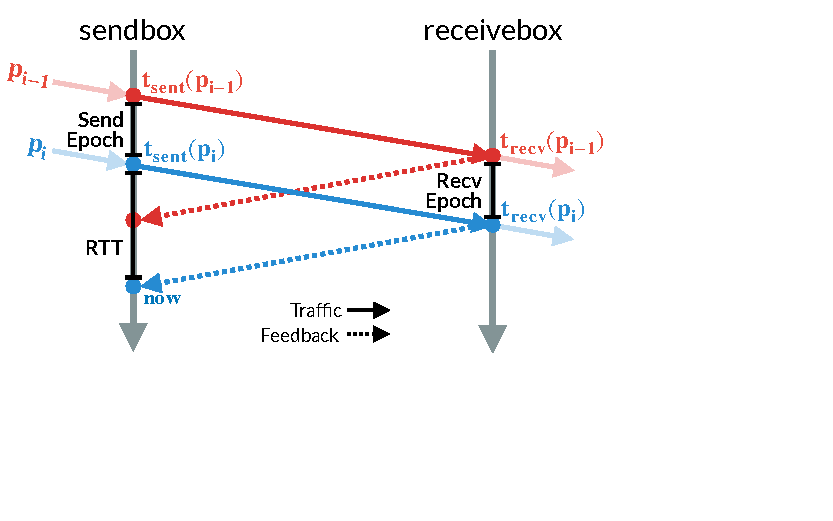
\includegraphics[width=\columnwidth]{img/rate-calculation}
    \caption{Epoch-based measurement calculation}\label{fig:ratecalc}
\end{figure}


\begin{outline}
\1 Packet marking for hands-off measurement
    \2 Congestion control protocols require accurate measurements for their decisions to be meaningful. How can an inbox and outbox collaborate to measure network conditions along their path?
    \2 Congestion control protocols need only a small, common set of measurements~\cite{ccp-hotnets} to function. We observe that these can be reconstructed with three core measurements: the sending rate at the in-box, the receiving rate at the out-box, and the round-trip time between the two gateways.
    \2 Unfortunately, to be most useful, the sending and receiving rates should be calculated over the same set of packets. Otherwise \an{why}.
        \3 Otherwise instantaneous measurements can't be used and everything has to be ewma'd?
    \2 We use packet flagging to synchronize these measurement epochs between the sender and the receiver.
    \2 Packet flagging is a technique where the inbox and outbox agree on some desired epoch length in packets.
    \2 Then, the inbox takes the hash of some field in the packet header (\eg TCP sequence number or IP ID).   
        \3 A suitable field should change with every packet (\ie, is not static for the lifetime of the connection).
        \3 On every packet p, given a desired epoch duration d, the inbox computes x = H(p) mod d where H is some hash function (which need not be cryptographically secure)
    \2 Epoch-based measurements
        \3 The inbox checks if x == 0. If it is, the inbox marks the start of a new epoch. It records the current time, and the cumulative number of bytes sent since some previous super-epoch.
        \3 Similarly, the outbox computes x = H(p) mod d on every packet. On a packet marking the start of a new epoch, the outbox sends an out-of-band packet to the inbox containing the hash of the epoch-marked packet, its current time, and the cumulative number of received bytes sent since the super-epoch.
        \3 When the inbox receives an out-of-band feedback message, it looks up that hash. If the packet which ended the previous epoch was sent at time $s_1$ and received at $r_1$, and the packet ending the current epoch was sent at time $s_2$ and received at $r_2$, the inbox can calculate:
            \4 rtt = current time - $s_2$
            \4 bytes in send epoch = bytes sent at s2 - bytes sent at s1
            \4 bytes in recv epoch = bytes sent at r2 - bytes sent at r1
            \4 send epoch duration = r2 - r1
            \4 received rate = bytes in recv epoch / recv epoch duration
        \3 Epoch durations are in expectation, since they depend on hash values.
    \2 The inbox now has relevant measurements, and can compute estimates of higher-level measurement primitives.
        \3 \eg loss rate = send rate - recv rate
\1 Suitable congestion control algorithms
    \2 Since \name cannot track low-level metrics used by traditional congestion control algorithms such as the number of inflight packets, implementations of window-based algorithms may not be suitable for use.
    \2 Fortunately there are rate-based algorithms available~\cite{bbr, nimbus}.
    \2 The inbox acts as a datapath for CCP~\cite{ccp}, and we use CCP implementations of BBR and Nimbus without modification.
\end{outline}